\section{Introduction}
\label{sec:introduction}

Long-context decoding rereads an increasingly long key--value (KV) history
for every generated token.  KV eviction reduces this cost by permanently
discarding states \citep{zhang2023h2o,li2024snapkv,cai2024pyramidkv,
feng2024adakv}; query-aware retrieval instead keeps all states addressable and
chooses a fresh subset at each step \citep{ribar2023sparq,tang2024quest,
singhania2024loki}.  Retrieval is useful only when selecting the subset costs
substantially less than the dense attention it replaces.

Low-bit token indices provide a direct selector: approximate all QK scores,
choose top-$k$, then apply exact attention to the original K/V.  FIER shows
that 1-bit Keys can retain useful rankings \citep{wang2025fier}, but a
uniform Key quantizer minimizes reconstruction error rather than the error
that attention observes,
$(q^\top k-q^\top\widehat k)^2$.  These objectives agree only for isotropic
Queries.  This motivates our central question: \emph{under a fixed index-byte
budget, how should representation capacity follow the joint Query--Key
geometry?}

We introduce \method, a training-free, GPU-resident exact-KV retrieval
method.  For each layer and KV head, prompt samples define two request-local
linear transforms.  The transforms are biorthogonal: before quantization they
preserve every dot product exactly, while both transformed second moments
equal the same diagonal joint-energy spectrum.  \method groups the 128
coordinates into eight 16-D bands and assigns each 0/1/2/4/8 bits by exactly
minimizing a separable bandwise logit-MSE surrogate under a 240-bit
token/head budget.
The resulting Key index adds 5.86\% to FP16 K+V storage.

At decode step $t$, a packed scan selects
\begin{equation}
 B(N)=\min\{N,1280,\max(256,\lceil0.06N\rceil)\}
 \label{eq:budget-intro}
\end{equation}
positions per Query head.  A sampled-quantile kernel avoids materializing an
$N$-length score vector or invoking generic top-$k$; original FP16 K/V then
receive exact sparse QK--softmax--AV.  There is no learned router, task rule,
exact-QK reranking, protected-token heuristic, or Full-attention fallback.

Selected-only attention can still fail when many individually small omitted
weights carry a coherent aggregate Value.  The frozen QKSieve-Robust consumer
therefore estimates the omitted partition and a current-Query rank-16 INT4
Value residual during the same scan, for 7.47\% total auxiliary storage.
QKSieve-Fast removes this residual and serves as the causal cost/quality
ablation; the main method does not switch profiles at a hand-set length.
\Cref{fig:overview} shows the complete path.

\begin{figure}[t]
  \centering
  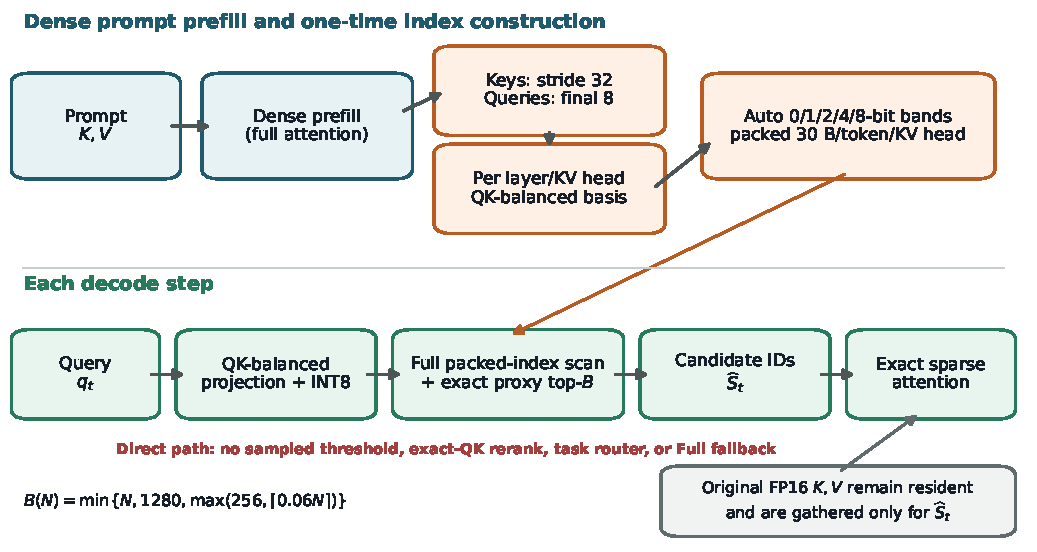
\includegraphics[width=\linewidth]{figures/qksieve_overview.pdf}
  \caption{\method builds request-local QK-balanced mixed-bit indices, scans
  them for each Query, and applies exact sparse attention to resident FP16
  K/V.  Robust also estimates the omitted Value tail; neither profile uses
  reranking or dense fallback.}
  \label{fig:overview}
\end{figure}

Our contributions are:
\begin{itemize}
  \item We derive full-rank QK-balanced coordinates that exactly preserve
  dot products and expose a joint score-energy spectrum, then formulate
  per-head mixed-bit indexing as a hardware-visible rate-distortion problem.
  \item We implement packed sampled-quantile selectors for GQA and MHA,
  followed by exact sparse attention, and introduce an explicit low-rank
  Value-tail correction for diffuse omitted mass.
  \item We connect quantization error to ranking and output error through
  exact factorization, logit-MSE, margin, omitted-mass, and residual bounds.
  \item We evaluate retrieval quality, full LongBench, native-128K stress
  cases, same-path FIER controls, directly timed attention and decode, and
  persistent-cache cold/warm/shared-prefix/append-only regimes.  The frozen
  Robust path reaches 99.805\% pooled 128K perplexity quality and
  1.08--4.12$\times$ native-MHA attention speedup from 8K to 128K.
\end{itemize}
